\section{Réflexions et réfractions sur le diamant}

\subsection{Réflexions}

L'objectif de cette partie était de trouver  différentes méthodes
de calcul de réflexion, afin d'avoir le meilleur réalisme visuel possible. \\

Dans une première approche, certes simpliste, mais rapide à mettre en œuvre,
nous avons utilisé une simple texture cubique. Cette méthode est extrêmement peu
coûteuse en performance, mais permet tout de même un rendu de qualité raisonnable
pour des objets simples. \\
Malheureusement, les diamants comportant des réflexions internes, cette méthode ne permet pas
de rendu convaincant, un rendu cubique autour de chaque face pouvant apporter des artefacts
visuels sur des faces adjacentes et proches.

Nous avons donc creusé dans une autre direction, en générerant, pour chaque triangle de la scène,
un rendu de son monde «~miroir~», dans un buffer commun à toute la scène.

Le but final est d'obtenir quelque chose ressemblant à ça~:

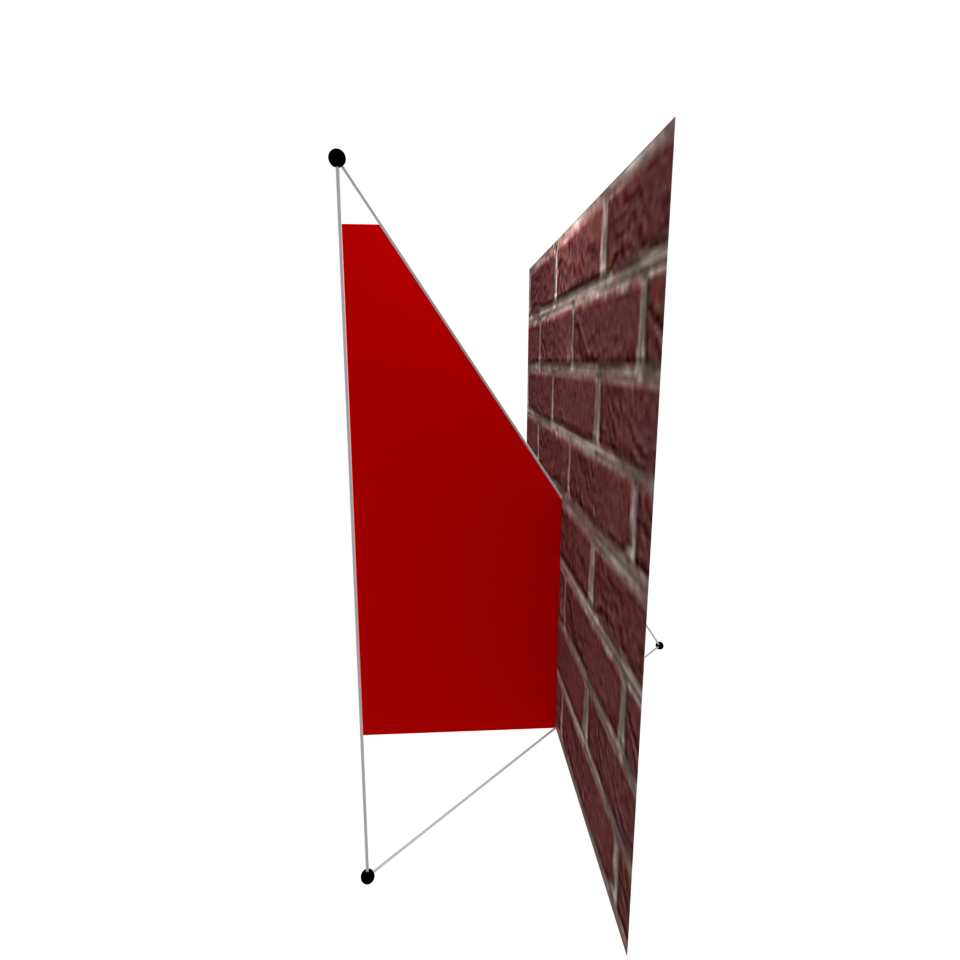
\includegraphics[width=0.45\textwidth]{Reflexion/6}

avec, en rouge, la zone où le rendu de la réflexion sera effectué.

Nous avons dans cet exemple un carré avec un miroir triangulaire tourné à 45°
par rapport au mur.

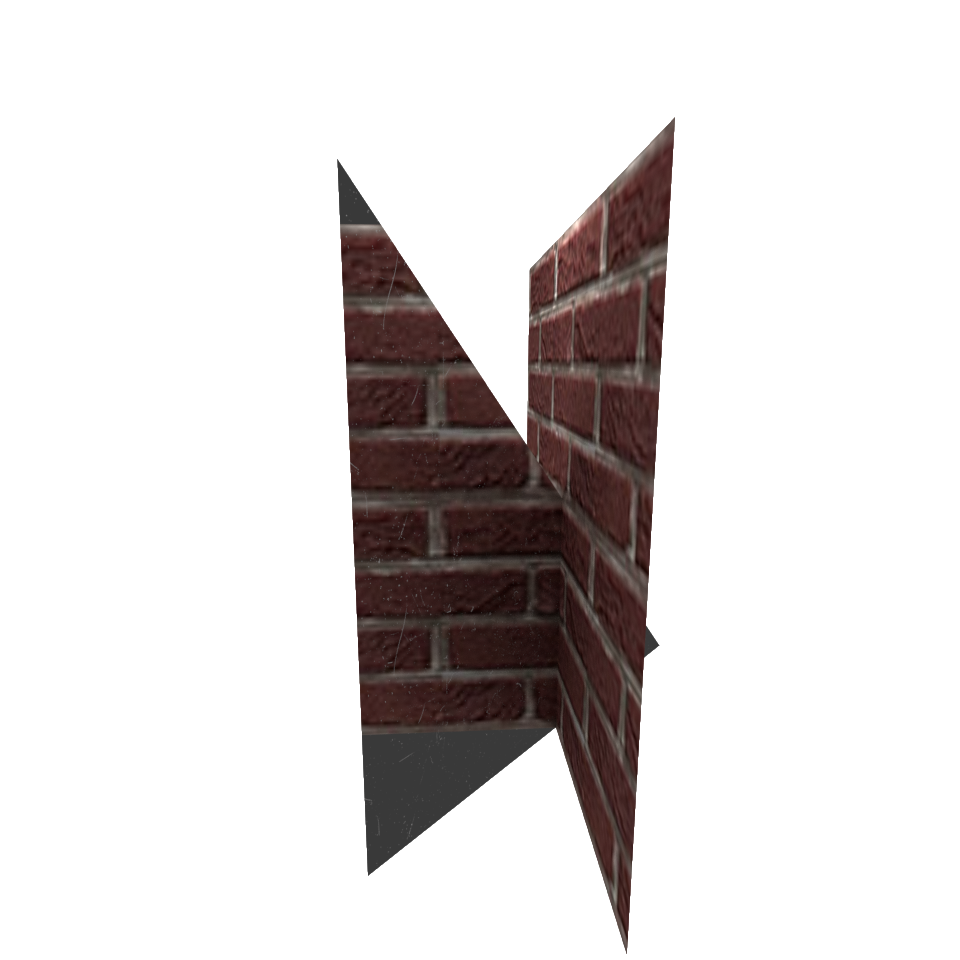
\includegraphics[width=0.45\textwidth]{Reflexion/1}

Pour chaque triangle se comportant comme un miroir on calcul la réflexion de la manière suivante~:

\begin{itemize}
    \item On récupère sa matrice Tangente – Bitangente – Normale (\textit{TBN}), qui nous permet
        d'effectuer la réflexion de la scène par rapport au triangle.

        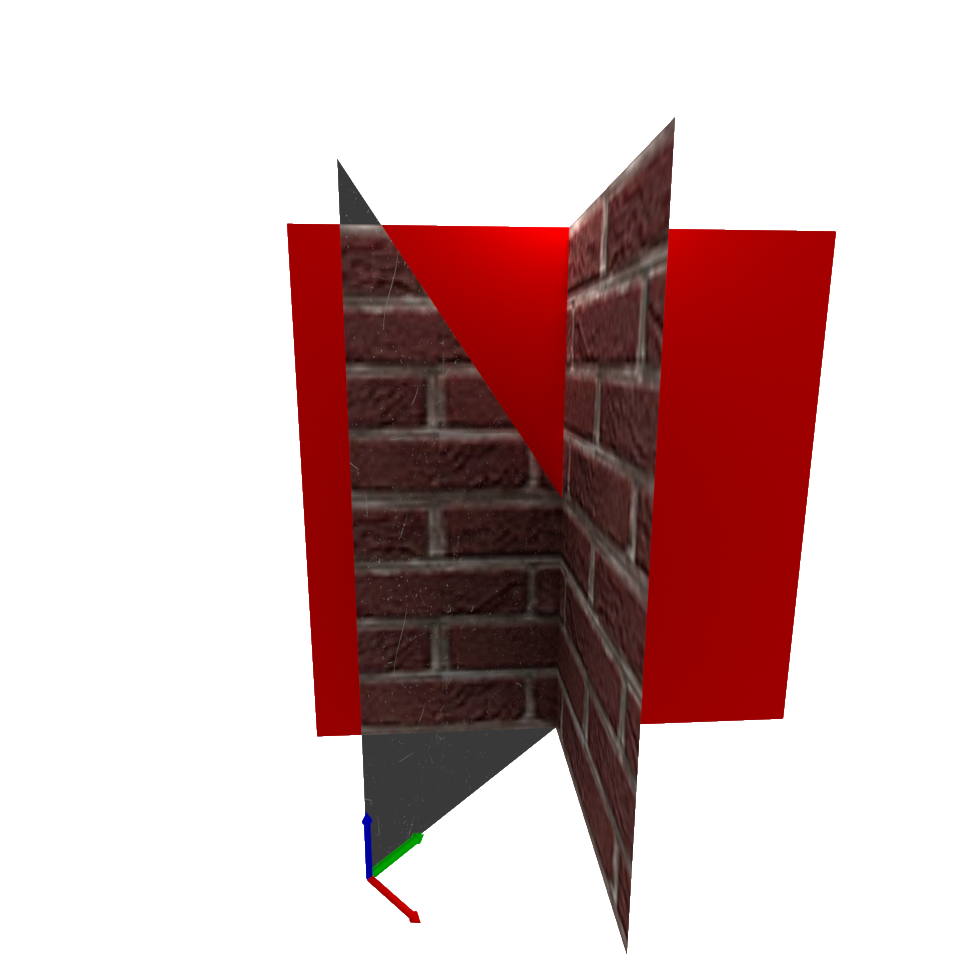
\includegraphics[width=0.45\textwidth]{Reflexion/3}

    \item On supprime ce qui se trouve de l'autre côté du mur ; en effet, une
        fois la réflexion effectuée, c'est uniquement la partie à l'avant qui
        représente le reflet.

        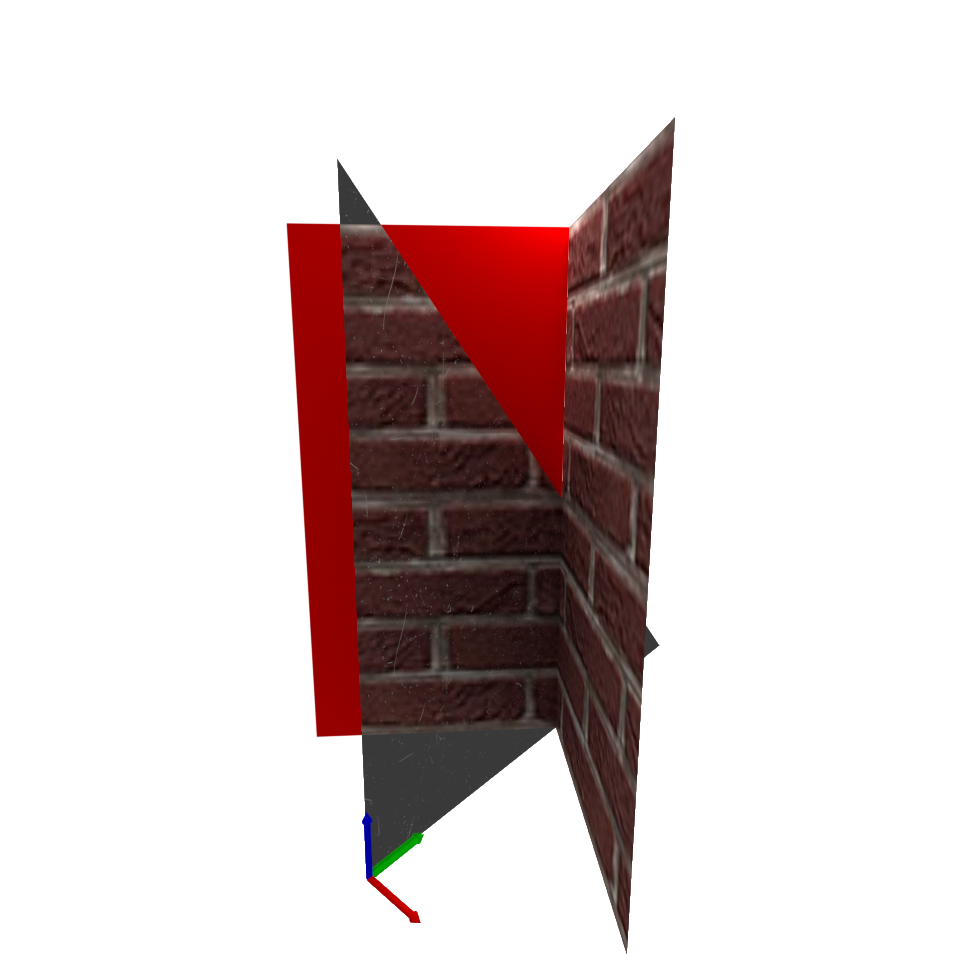
\includegraphics[width=0.45\textwidth]{Reflexion/4}
        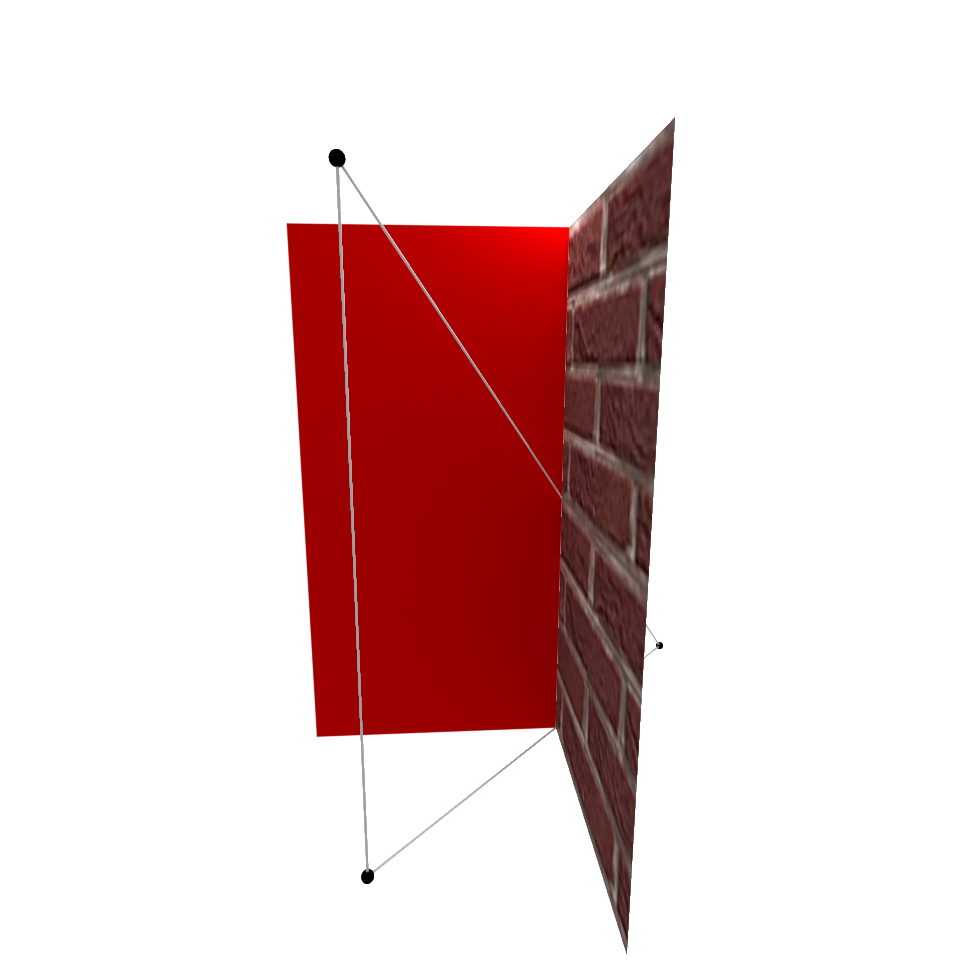
\includegraphics[width=0.45\textwidth]{Reflexion/5}
    \item Et pour finir, on ne garde que les pixels se trouvant à l'intérieur
        du triangle que l'on est en train de rendre.

        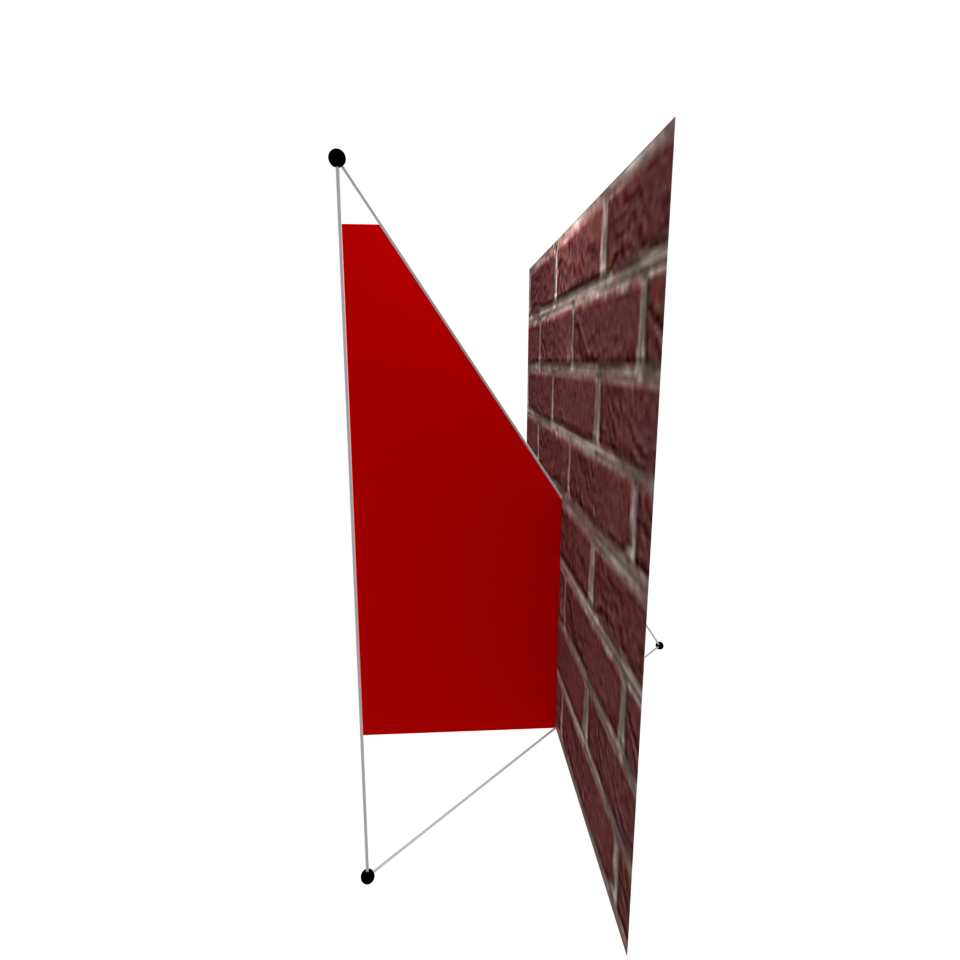
\includegraphics[width=0.45\textwidth]{Reflexion/6}
\end{itemize}

\subsection{Réfractions}

Pour calculer les réfractions, il y a une étape supplémentaires car la lumière est dispersée,
mais est également décomposée, en fonction de l'angle d'incidence et du matériau.

On a choisi ici de traiter l'image comme le ferait une vraie caméra, c'est à dire
avec trois canaux de couleur.
On peut alors soit effectuer chaque rendu trois fois, soit rendre de manière séparée le bleu,
le vert, et le rouge. Chaque réfraction dépendra donc de la matrice \textit{TBN} de la
surface, et de son indice de réfraction (le rapport entre l'angle d'incidence et l'angle réfracté),
mais également de la longueur d'onde de la lumière en train d'être rendue.

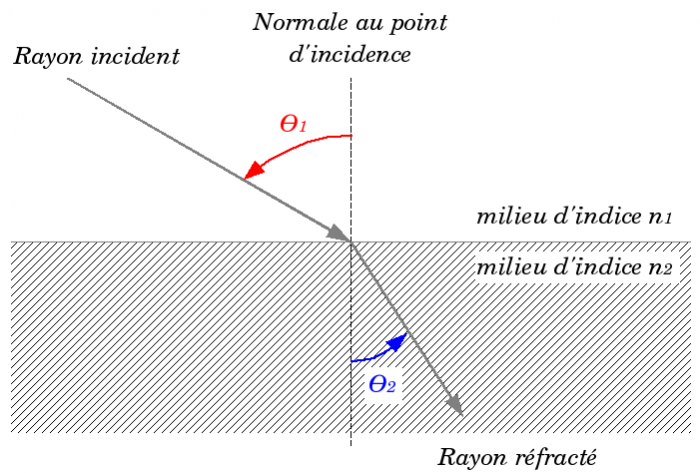
\includegraphics[width=0.65\textwidth]{Refraction/refraction}

Les étapes suivantes pour cette partie sont les mêmes que pour la réflexion.

Il suit ensuite des étapes plus complexes, qui n'ont malheureusement pas été implémentées.
En effet, il reste les étapes de récurrences, qui permetteraient de voir les
réflexions/réfractions se propager sur plusieurs faces,
la profondeur de réflexion étant paramétrable.

Ces rendus supplémentaires ne sont pas triviaux, car un rendu de réflexion et de réfraction
supplémentaire est nécessaire pour chaque niveau de récursiviter, combinant les textures lors
d'un reflet double (comme par exemple un mirroir qui se reflète dans un autre mirroir), le tout
en prenant en compte l'angle d'incidence, via l'utilisation du Fresnel.

Cette méthode est très coûteuse en termes de performance,
mais notre but étant le réalisme, elle pourrait s'avérer satisfaisante.

\subsection{Résultat actuel}

Nous n'avons pas eu le temps d'implémenter la réfraction et la récursivité, mais
la réflexion est bien fonctionnelle dans le logiciel. La figure suivante
montre le résultat.

{\centering 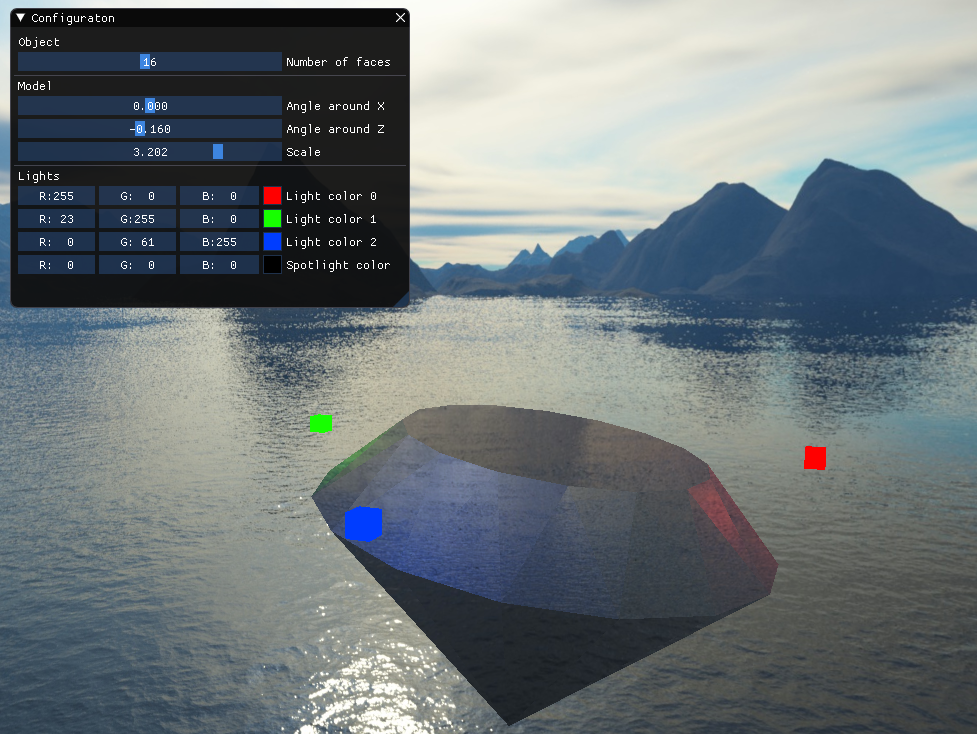
\includegraphics[width=0.9\textwidth]{screenshot_software_4}}

